\documentclass[10pt,twocolumn,letterpaper]{article}

\usepackage{cvpr}
\usepackage{times}
\usepackage{epsfig}
\usepackage{graphicx}
\usepackage{amsmath}
\usepackage{amssymb,bbm,xcolor}
\usepackage[breaklinks=true,bookmarks=false]{hyperref}
\usepackage{lipsum}
\usepackage{listings}
\usepackage{booktabs, multicol, xcolor}
\usepackage[shortlabels]{enumitem}
\usepackage{changepage}
\cvprfinalcopy % *** Uncomment this line for the final submission
\setcounter{page}{1}
\renewcommand{\figurename}{Figure}

\begin{document}
\title{Optimization for Data Science - Homework 1}
\author{Chiara Bigarella\\{\tt\footnotesize Student nr. 2004248}\and Silvia Poletti\\{\tt\footnotesize Student nr. 1239133}\and Gurjeet Singh\\{\tt\footnotesize Student nr. 2004251}\and Francesca Zen\\{\tt\footnotesize Student nr. 2010640}}
\maketitle

\section{Introduction}
The goal of this simulation is to explore and compare the performances of the Gradient Descent method and the Block Coordinate Gradient Descent methods with randomized and cyclic rules, in Semi-Supervised Learning. For this purpose, we will first consider a convex function minimization problem with respect to randomly generated points in the 2D space. Secondly, we will approach the same problem on a real-world dataset. In particular, the classification task is carried out by examining the feature similarities of the data.

\section{Materials}
The preliminary part of the simulation focuses on the binary classification of random points in the 2D space.\\ 
In the second part of our work, we consider a balanced subset of the HTRU2 dataset\footnote{https://archive.ics.uci.edu/ml/datasets/HTRU2}, containing a sample of Pulsar candidates, labeled as Pulsar or Non-Pulsar stars. Each Pulsar candidate is described by some continuous statistic measures (mean, standard deviation, kurtosis and skewness) of the integrated profile and the DM-SRN Curve, for a total of eight features. Data is pre-processed with standardization in order to reduce the variability of the features.\\

The binary classification task is carried out in Semi-Supervised Learning on a small number of labeled examples $(\bar{x}^{i}, \bar{y}^{i})$ for $i=1,...,l$, with labels in $\{-1,1\}$, and a vast number of unlabeled examples $x^{j}$ for $j=1,...,u$. The goal is to find the optimal labels $y^{j}$ associated to $x^{j}$ such that:
\begin{equation}\label{eqn:loss}
	\min_{y\in \mathbb{R}^{u}} \sum_{i=1}^{l} \sum_{j=1}^{u} w_{ij}(y^{j}-\bar{y}^{i})^{2} + \frac{1}{2}\sum_{i=1}^{u}\sum_{j=1}^{u} \overline{w}_{ij}(y^{i}-y^{j})^{2}.
\end{equation} 
In particular, \mbox{$W=[w_{ij}]_{\begin{subarray}{l}\text{$i=1,...,l$}\\ \text{$j=1,...,u$}\end{subarray}}$ and $\overline{W}=[\overline{w}_{ij}]_{\begin{subarray}{l}\text{$i=1,...,u$}\\ \text{$j=1,...,u$}\end{subarray}}$} are the similarity matrices whose components can be respectively interpreted as follows:
\begin{itemize}
	\item $w_{ij}$ expresses the similarity between the labeled example $\bar{x}^{i}$ and the unlabeled example $x^{j}$;
	\item $\overline{w}_{ij}$ expresses the similarity between the unlabeled examples $x^{i}$ and $x^{j}$.
\end{itemize}
The components of matrix $W$ (and similarly for matrix $\overline{W}$) can be defined by using one of the following Euclidean distance-based similarity measures:
\begin{enumerate}[(I)]
	\item $\displaystyle w_{ij} = \frac{1}{1+\lVert x^{j} - \bar{x}^{i} \rVert_{2}}$, where adding 1 to the Euclidean distance at the denominator imposes an upper bound of 1 to the value of $w_{ij}$;
	\item $\displaystyle w_{ij} = \exp\bigg(\frac{-\lVert x^{j} - \bar{x}^{i} \rVert_{2}^{2}}{2\sigma^{2}}\bigg)$, where the smaller $\sigma^2$ the faster the decreasing of $w_{ij}$ for increasing values of the Euclidean distance.
\end{enumerate}
It's important to notice that these measures take values in the range of $[0,1]$ and higher values occur when the data samples are more alike, i.e. when their Euclidean distance is lower. Therefore, problem \eqref{eqn:loss} gives higher priority to the minimization of the terms associated to the higher similarity weights $w_{ij}$ and $\overline{w}_{ij}$: if two points are assigned with a high similarity value, then their labels will be forced to be equal, with a higher priority with respect to couples of points associated to low similarity values.\\
Moreover, the similarity matrices are made sparse by applying a threshold on the components: in this way we avoid the exploding gradient problem (overflow) because similarity values that are not close enough to 1 are set as 0.\\

For simplicity, we can rewrite the objective function of problem \eqref{eqn:loss} by exploiting the fact that $\overline{w}_{ij} = \overline{w}_{ji}$:
\begin{flalign}
	f(y) &= \sum_{i=1}^{l} \sum_{j=1}^{u} w_{ij}(y^{j}-\bar{y}^{i})^{2} + \frac{1}{2}\sum_{i=1}^{u}\sum_{j=1}^{u} \overline{w}_{ij}(y^{i}-y^{j})^{2}&&\\ \nonumber
	& = \sum_{i=1}^{l} \sum_{j=1}^{u} w_{ij}(y^{j}-\bar{y}^{i})^{2} + \sum_{i=1}^{u}\sum_{j=i}^{u} \overline{w}_{ij}(y^{i}-y^{j})^{2}.
\end{flalign} 
Then, the j-th component of the gradient results to be:
\begin{flalign}
	\nabla_{y^{j}}f(y) &= 2 \sum_{i=1}^{l} w_{ij}(y^{j}-\bar{y}^{i}) - 2 \sum_{i=1}^{u}\overline{w}_{ij}(y^{i}-y^{j})&&\\ \nonumber
	& = 2 \sum_{i=1}^{l} w_{ij}(y^{j}-\bar{y}^{i}) + 2 \sum_{i=1}^{u}\overline{w}_{ij}(y^{j}-y^{i}).
\end{flalign}
\\
\section{Methods}
The classic Gradient Descent (GD) method calculates each iterate as 
\begin{equation}
	y_{k+1} = y_k - \alpha_k \nabla f(y_k)
\end{equation}
with stepsize $\alpha_k>0$.\\
The convergence rate of the GD method is dimension-free, but the computation of the full gradient can be very costly when dealing with high-dimensional data. \\

On the other hand, the idea underlying the Block Coordinate Gradient Descent (BCGD) methods is to split the optimization problem into smaller optimization processes by assuming that the variables are partitioned in $b$ blocks of dimension $n_i$, for $i=1,...,b$, such that $u = n_1 +\dots + n_b$, where $u$ is the dimension of our problem. In our case: $n_i = 1$ and $b = u$.\\ 
In particular, the Cyclic BCGD method updates each iterate only after computing
\begin{equation}
	y_i = y_{i-1} - \alpha_i U_i \nabla_{i} f(y_{i-1})
	\label{BCGD_equation}
\end{equation}
for each block $i$, where $\mathbb{I} = [U_1| \dots | U_b]$ is the identity matrix in $\mathbb{R}^{n \times n}$.\\
Instead, the Randomized BCGD method calculates each iterate as 
\begin{equation}
	y_{k+1} = y_{k} - \alpha_k U_{i_k} \nabla_{i_k} f(y_{k})
\end{equation}
where block $i_k$ is randomly chosen at each iteration, by sampling from the uniform distribution, i.e. $P(i_k = i) = \frac{1}{u}\;\;\; \forall \; i=1...u$.\\

\section{Results}
All the methods have been implemented by setting a fixed stepsize, since the complexity of Exact Line Search or Armijo Rule results to be prohibitive in practice: our objective function is neither cheap nor well structured, because it can't be fully rewritten in matrix form.

For what concerns the stopping criterion, all the methods are forced to not exceed the number of maximum iterations and GD and Cyclic BCGD are also forced to stop when the norm of the gradient gets lower than a certain tolerance. This last condition is not applied to Randomized BCGD because we noticed that the quantity $|u \cdot \nabla^2_{i_{k}}f(y_k)|$ is not enough representative of the full gradient norm. Moreover, for computational complexity reasons, we excluded the stopping criterion based on the value of the loss function.

Since the optimization problem (\ref{eqn:loss}) is defined for $y\in\mathbb{R}^u$, we also define the iterates of all the methods as real-valued vectors and the resulting gradient norm at the optimum is very close to 0. \\
Then, to assess the classification task for $y\in\{-1,1\}^u$ we discretize the optimum by considering $sign(y)$ and compute again the gradient on this discrete vector. The norm of the new gradient is reasonably higher than the one of the gradient computed on the real-valued optimum. Indeed if the components of $y$ assume only values equal to -1 or 1, then the terms $(y^i - \bar{y}^i)$ and $(y^i - y^j)$ can be only equal to -2, 0 or 2; therefore, the final sum is reasonably very high in absolute value. On the contrary, if $y$ is continuous, the previous terms can assume values in a range of $[-2, 2]$, thus the final sum is reasonably closer to 0.\\
In particular, a smaller value of the gradient computed on $sign(y)$ always corresponds to a better accuracy, while this is not always the case for the gradient computed on $y$.

\subsection{Toy Example}
To start, we consider a balanced toy example of 400 labeled and 1000 unlabeled datapoints, generated from two Gaussian distributions with same variance but different means, as represented in Figure \ref{fig:toy_example}.\\
\renewcommand{\thefigure}{1}
\begin{figure}[htbp]
	\centering
	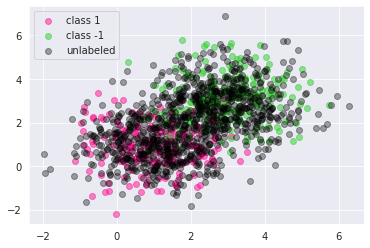
\includegraphics[width=6.5cm]{img/scatter_toy}
	\caption{Toy example 2D plot.}
	\label{fig:toy_example}
\end{figure}
\renewcommand{\thefigure}{3}
\begin{figure*}[t]
	\centering
	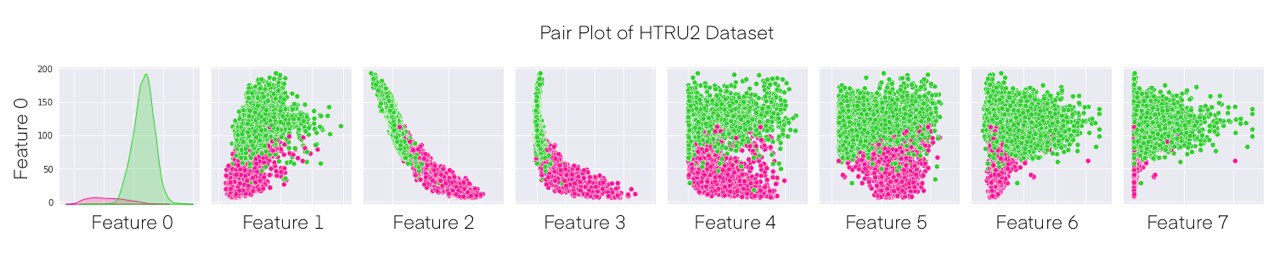
\includegraphics[width=15cm]{img/sep}
	\caption{HTRU2 Features Pair Plots}
	\footnotesize{This figure shows just the first row of the Pairs Plot of HTRU2 Dataset, representing the first feature in relation to all the other seven features. We can find the density curves on the diagonal, representing the distribution of a single variable, and the scatter-plots on the upper and lower triangles, showing the relationship between two variables. \\ Class 1 (Pulsar) is colored in pink and Class -1 (Non-Pulsar) in green. }
	\label{fig:sep}
\end{figure*}

The Gaussian Radial Basis function (similarity measure II) with $\sigma^2$ equal to the variance of the two Gaussian distributions, empirically shows to work well.\\

Figure \ref{fig:gradient} shows almost the same smooth gradient decreasing for the GD and the Cyclic BCGD, while the Randomized BCGD produces a much more irregular decreasing, since it modifies just one component of $y$ at each iteration.
\renewcommand{\thefigure}{2}
\begin{figure}[htbp]
	\centering
	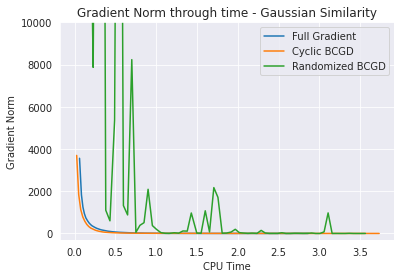
\includegraphics[width=6.5cm]{img/gradplot_cropped}
	\caption{Gradient norm vs CPU time (cropped plot).}
	\label{fig:gradient}
\end{figure}

As shown in Table \ref{tab:toy}, the Randomized BCGD is the fastest method because the calculation of the partial derivatives is much cheaper than computing the whole gradient, but, for the same reason, it requires much more iterations to converge: in order to pass through all of the $u$ blocks at least one time, it needs much more then $u$ random attempts.\\

\begin{table}[h]
	\begin{center}
	\begin{adjustwidth}{-1.3cm}{}
	\begin{tabular}{lrrr}
	{} &          GD &      Cyclic &     Randomized \\
	\midrule
	Gradient on y       &    0.05012 &    0.04985 &       0.82172 \\
	Gradient on sign(y) &  660.94980 &  660.92631 &     660.92631 \\
	Iterations          &  636 &  626 &  150000 \\
	CPU time            &   11.85532 &   15.42657 &       9.74568 \\
	Accuracy            &   91.90 &   92.00 &      92.00 \\
	\end{tabular}
	\end{adjustwidth}
	\end{center}
	\caption{Toy example Summary.}
	\label{tab:toy}
\end{table}
Moreover, Cyclic BCGD computes $u$ partial gradients at each iteration, while GD directly computes the full gradient of length $u$; since the computational complexity of BCGD methods depends on the number of blocks (and here we consider $b=u$) then Cyclic BCGD needs slightly fewer iterations but higher CPU time than GD to converge.\\
In conclusion, all the three methods are able to reach an accuracy of almost 92\%.
\subsection{HTRU2 Dataset}
Since the HTRU2 dataset is strongly unbalanced, we selected a balanced subset composed by 800 labeled and 1500 unlabeled datapoints.\\
This dataset is particularly suitable for our application because the features of the datapoints are almost linearly separable, as shown in Figure \ref{fig:sep}. Therefore Euclidean distances are well representative of the feature similarities. Instead, in case of a dataset in which points from different classes widely overlap, we may have many points that are close to each other but are not similar.

Results in Table \ref{tab:dataset} are coherent with the theory: random sampling improves the convergence rate expectation, but results to be highly time-consuming in large-scale problems. Indeed, here we're considering a bigger dataset than the previous toy example. \\ 
\begin{table}[h]
	\begin{center}
		\begin{tabular}{lrrr}
			{} &          GD &      Cyclic &     Randomized \\
			\midrule
			Gradient on y       &    0.50122 &    0.49961 &       3.13508 \\
			Gradient on sign(y) &  238.53269 &  238.32253 &     238.83703 \\
			Iterations          &  582 &  578 &  250000 \\
			CPU time            &   20.23947 &   26.04186 &      20.92415 \\
			Accuracy            &   89.40 &   89.47 &      88.40 \\
		\end{tabular}
	\end{center}
	\caption{HTRU2 Summary.}
	\label{tab:dataset}
\end{table}
\pagebreak

In Figure \ref{fig:accuracy} we can see the accuracy of the methods through the time needed by each method to reach the minimum. It is interesting to notice that GD and Cyclic BCGD methods reach a good accuracy in very few steps while Randomized BCGD method needs some extra time.

\renewcommand{\thefigure}{4}
\begin{figure}[htbp]
	\centering
	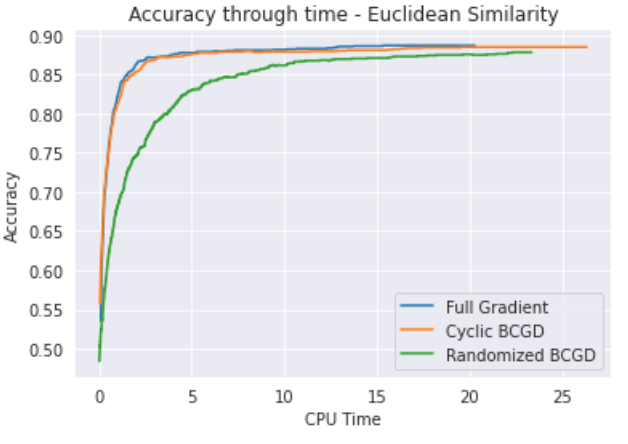
\includegraphics[width=7cm]{img/accuracy}
	\caption{Accuracy vs CPU time. }
	\label{fig:accuracy}
\end{figure}

\section{Conclusions}
Switching from the toy example to the real-world dataset increased the amount of data points and with them the CPU time required for the three methods to converge, while the accuracy slightly drops.

In particular, our empirical results confirm the fact that the Cyclic BCGD  iteration cost is $\mathcal{O}(b)$ times larger than Randomized BCGD.\\

While the Randomized BCGD seems the best choice for small-dimensional problems, it is sligthly slower compared to the classic Gradient Descent method in larger-scale problems.

In general, the BCGD methods would perform better when considering bigger blocks, a non-fixed stepsize and a strongly convex function. In our work, each block has dimension 1, thus we are not exploiting any structure and the stepsize is fixed, so Cyclic BCGD takes more or less the same iterations as GD to converge. Moreover, Randomized BCGD should improve a lot when considering non-uniform sampling.



%The randomized BCGD method had better performance on the former set of points, and this can be seen either on the CPU time and on the number of iterations. On the other hand GD and Cyclic BCGD methods DA COMPLETARE
\end{document}
